\chapter{Design Method Example: Electrical Power Subsystem}\label{CH:Design2}

This subsystem was designed to facilitate expanded capabilities of the IT-SPINS mission. Building on successes of the electrical power subsystem (EPS) used for the FIREBIRD-II mission, the design of an updated version of the Phoenix EPS began in the Spring of 2016. The original design came out of necessity, and began a trend of using SSEL developed subsystems for CubeSat missions rather than purchasing and integrating off-the-shelf solutions. 

This chapter provides an investigation of how IT-SPINS mission requirements made a significant overhaul of the Phoenix EPS mandatory. Then, a conceptual design that incorporates those requirements is presented. With a block diagram in place, several circuit simulations and calculations were performed to verify that components of the design would operate as intended once built. The method used in this example effectively used a hierarchical schematic structure to reuse several ``blocks'' and make the schematic less cluttered. However, simulations were not well integrated into the design flow and were difficult to track as the design matured; if a simulation was modified or updated the corresponding schematic changes had to be done manually. Similarly, support documents such as connector pin reference tables were in a constant state of flux as the design progressed.

Figure~\ref{fig:eps_flow} is an overview of the processes involved in designing the Phoenix EPS. Ideally, these steps would be linked in only a linear progression, i.e. each step would need to be completed and approved before moving onto the next. The arrows show that during the simulation and schematic entry phases there was a need to revise the subsystems requirements and conceptual design material. Also, there was essentially only one formal approval step, made when the PCB was fully laid out and ready for fabrication.

\begin{figure}[htbp]
	\centering
	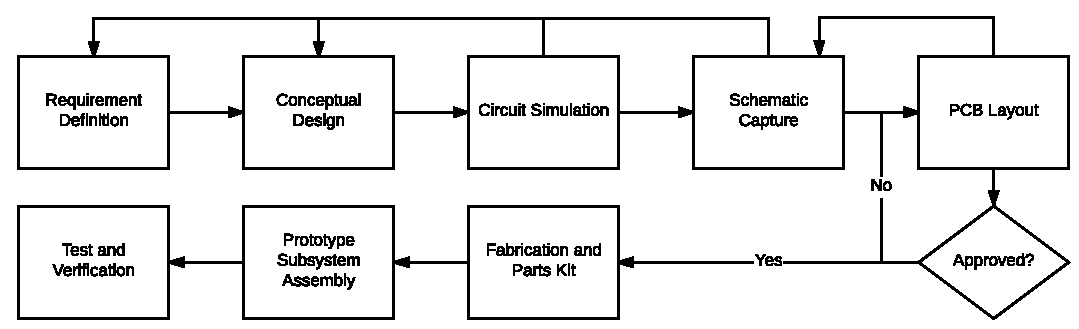
\includegraphics[width=\textwidth]{../figs/phoenix/concept/eps_flow.pdf}
	\caption{A simplified representation of the design method used in this chapter.}
	\label{fig:eps_flow}
\end{figure}

\section{Requirements and Conceptual Design}\label{Sect:eps_concept}

\begin{figure}[htbp]
	\centering
	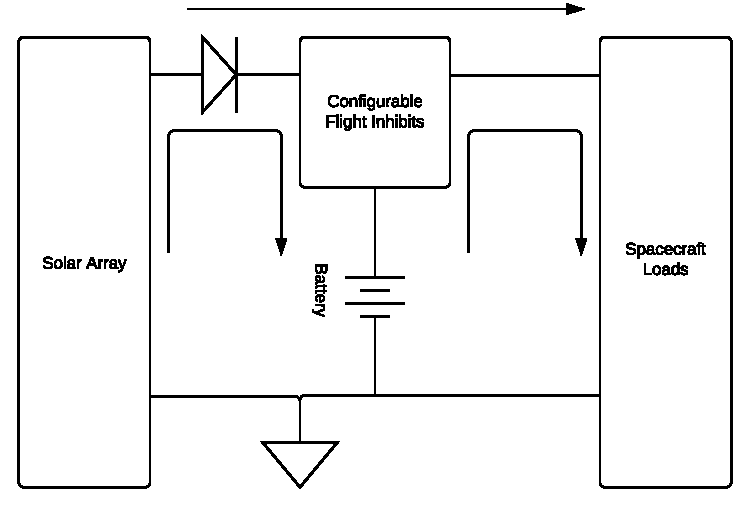
\includegraphics[width=0.7\textwidth]{../figs/phoenix/concept/eps_basic.pdf}
	\caption{Basic configuration of a direct energy transfer (DET) power subsystem, with primary current paths shown by arrows.}
	\label{fig:eps_basic}
\end{figure}

\begin{figure}[htbp]
	\centering
	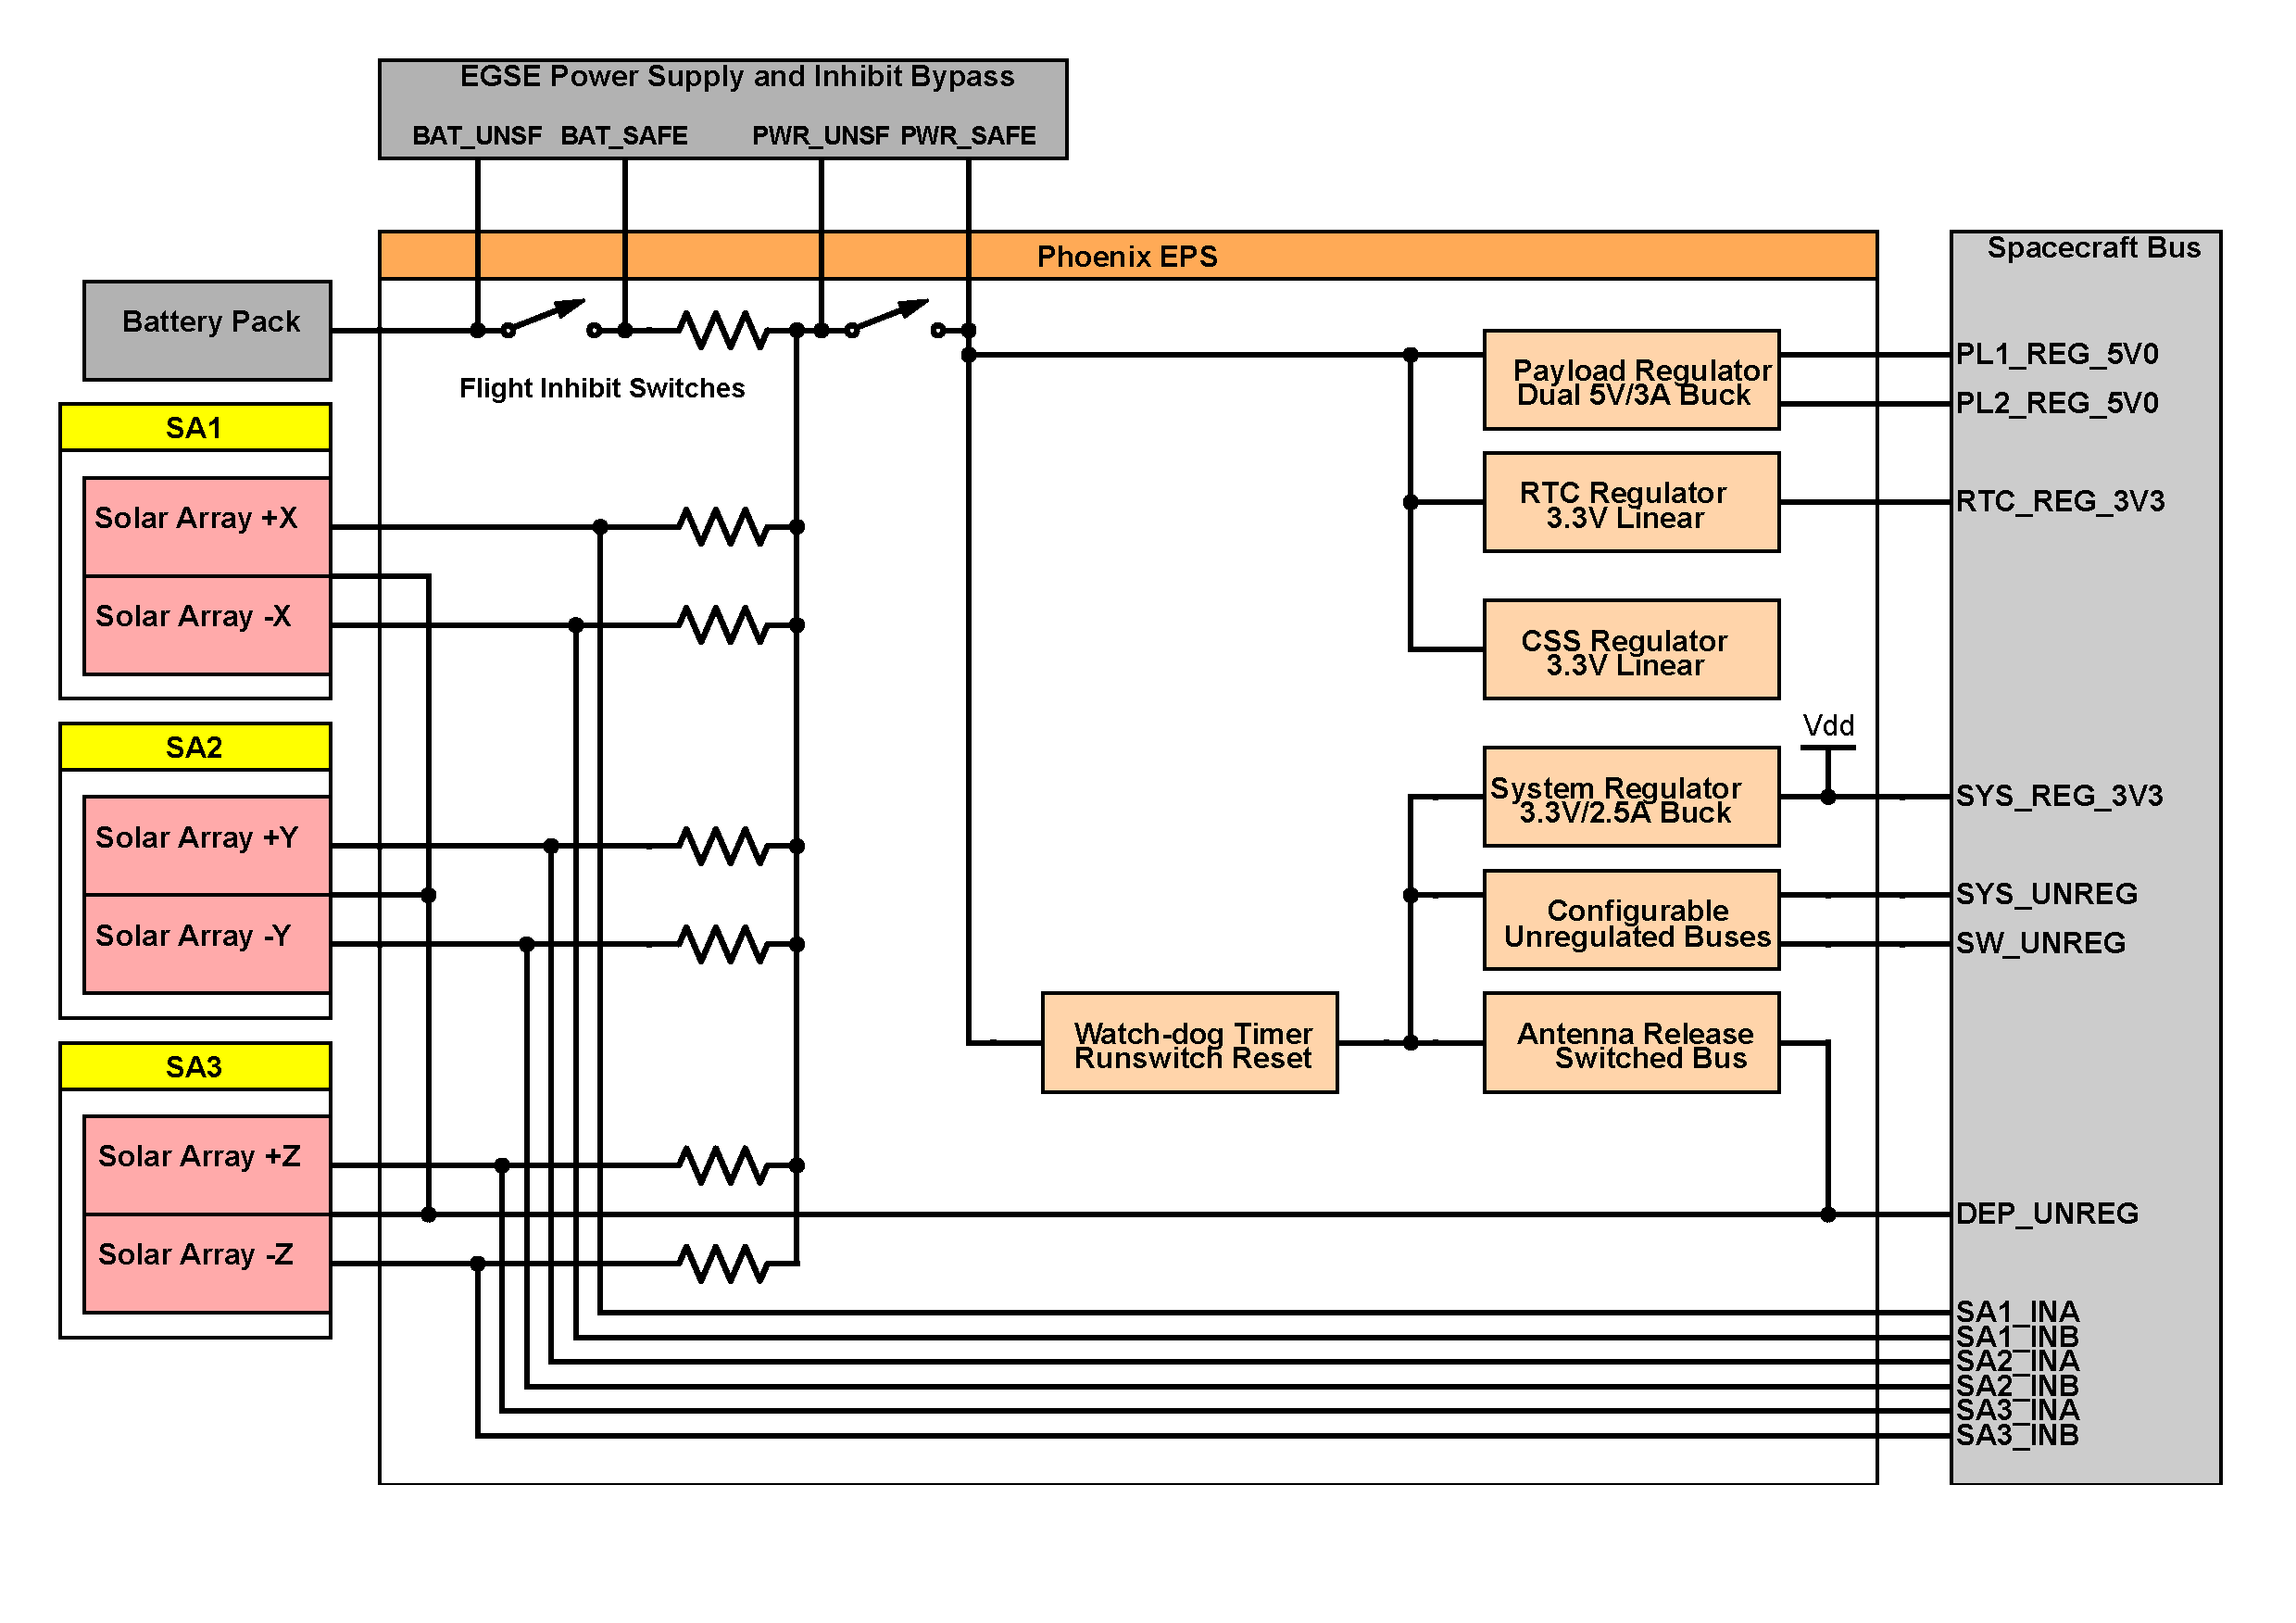
\includegraphics[width=\textwidth]{../figs/phoenix/concept/system_diagram.pdf}
	\caption{Components of the Phoenix EPS and the connections that form the PDN of the spacecraft.}
	\label{fig:eps_block}
\end{figure}

Each resistor shown indicates a critical current sense location that is used to monitor the subsystem's status and performance. The inhibit switches shown indicate the locations at which the power path is broken for ``safing'' the satellite during test and launch; the physcial switches are not located on the

\begin{figure}[htbp]
	\centering
	%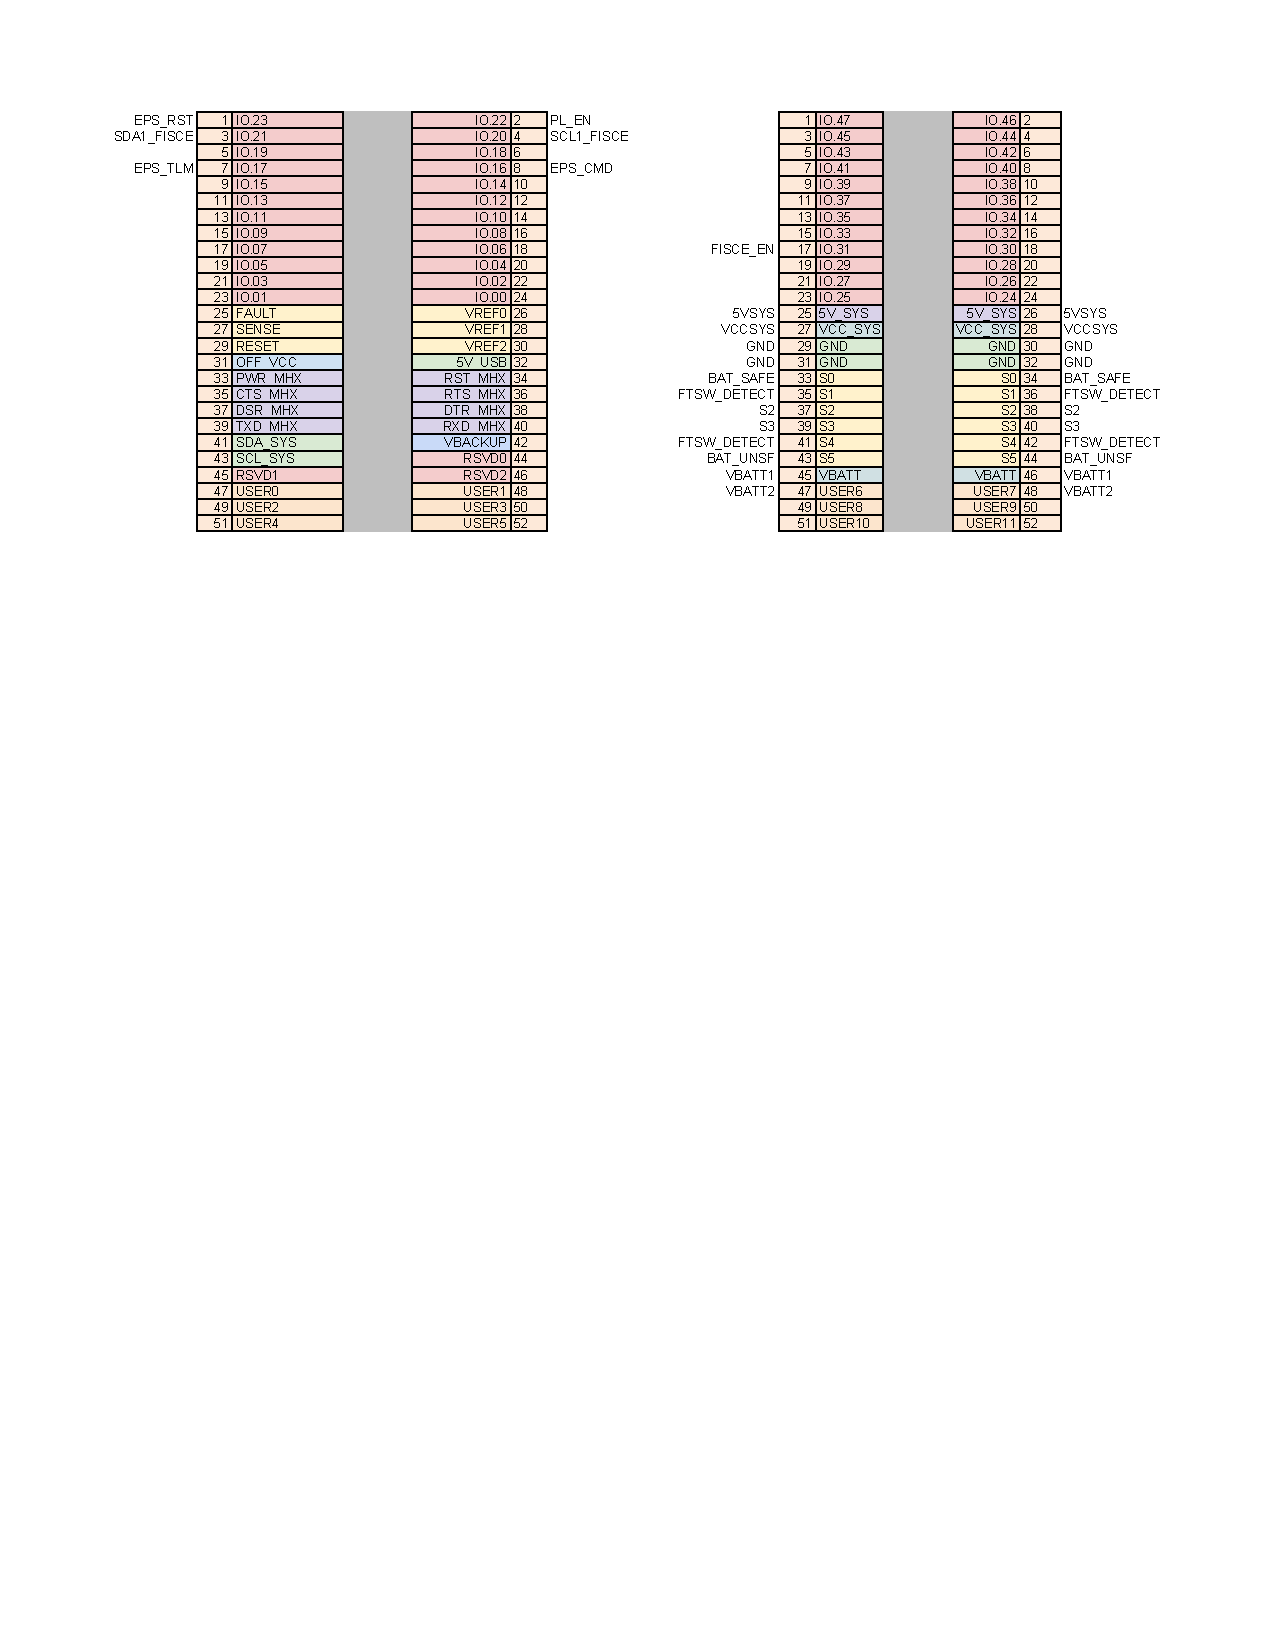
\includegraphics[width=\textwidth]{../figs/phoenix/concept/old_bus.pdf}
	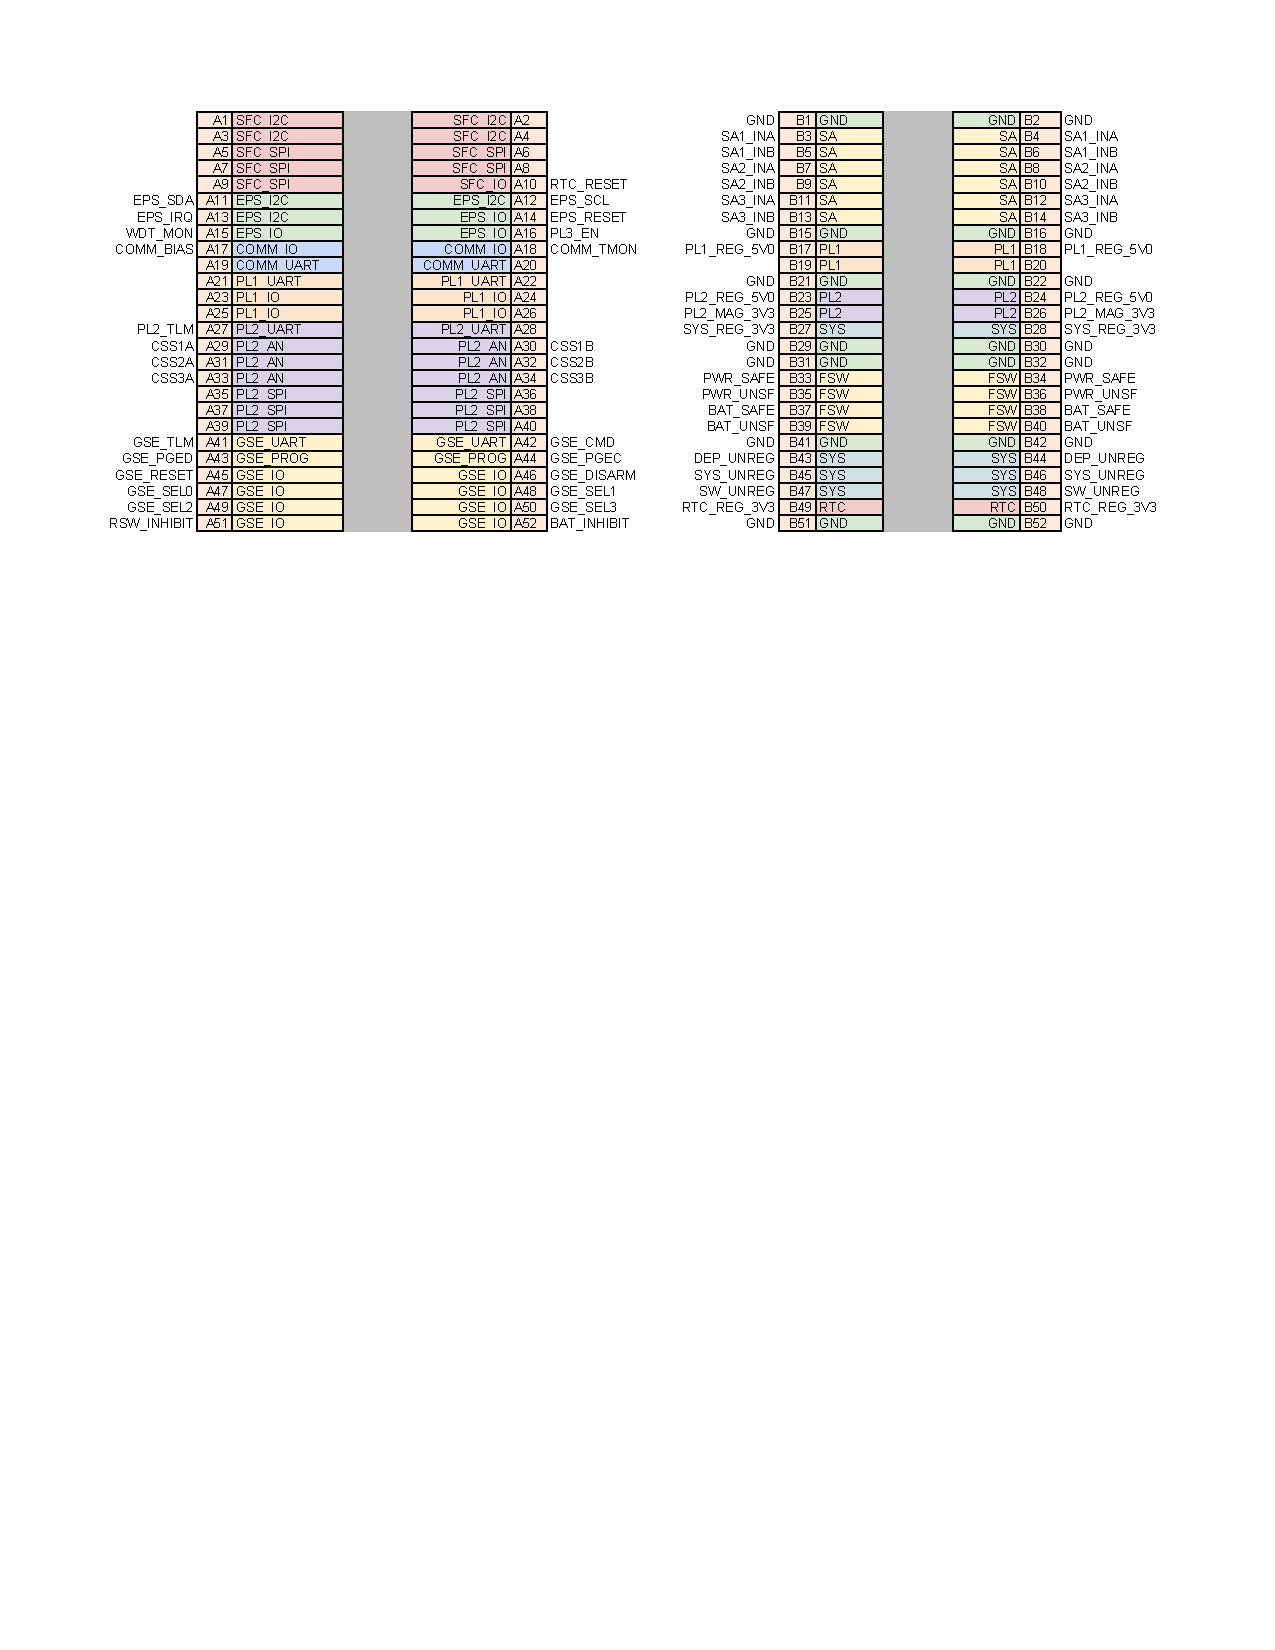
\includegraphics[width=\textwidth]{../figs/phoenix/concept/new_bus.pdf}
	\caption{New connector pinouts.}
	\label{fig:eps_bus}
\end{figure}

\begin{figure}[htbp]
	\centering
	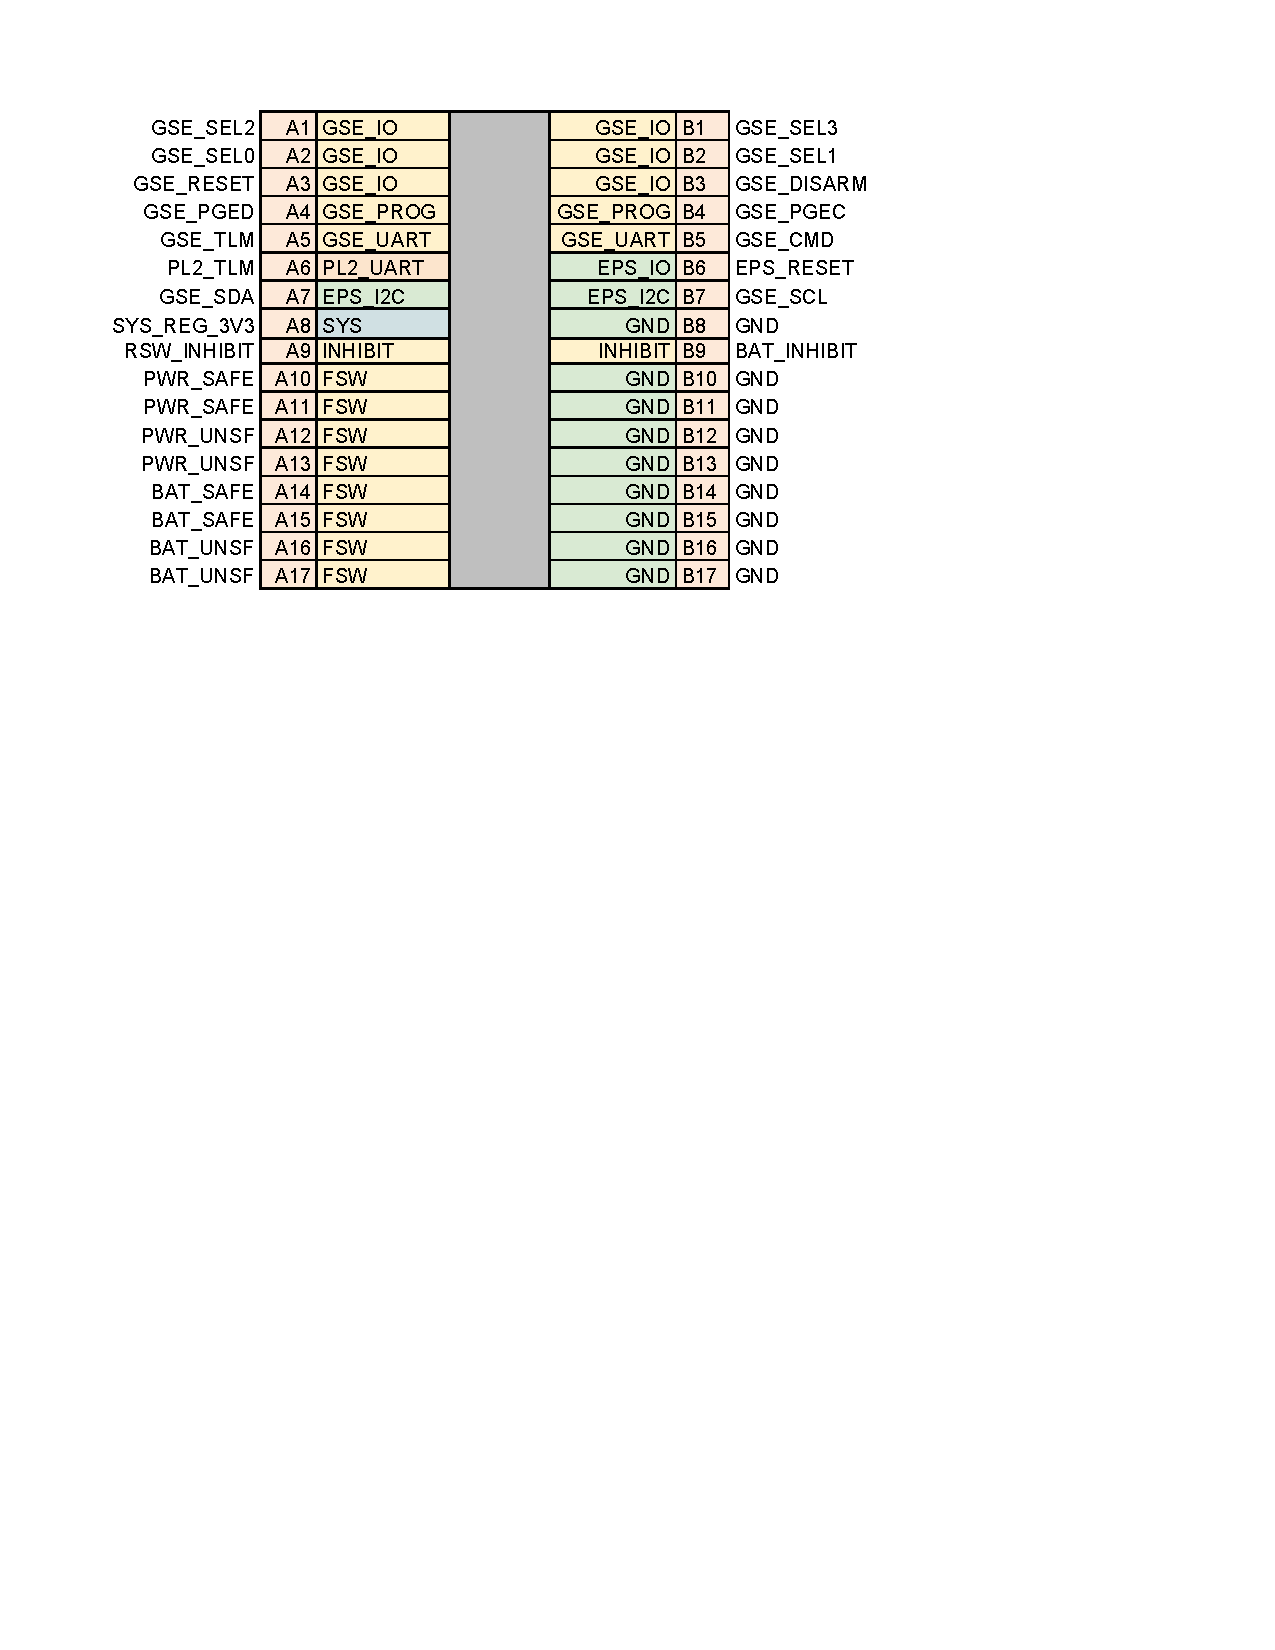
\includegraphics[width=0.5\textwidth]{../figs/phoenix/concept/egse_pins.pdf}
	\caption{New connector pinouts.}
	\label{fig:egse_pins}
\end{figure}

\begin{figure}[htbp]
	\centering
	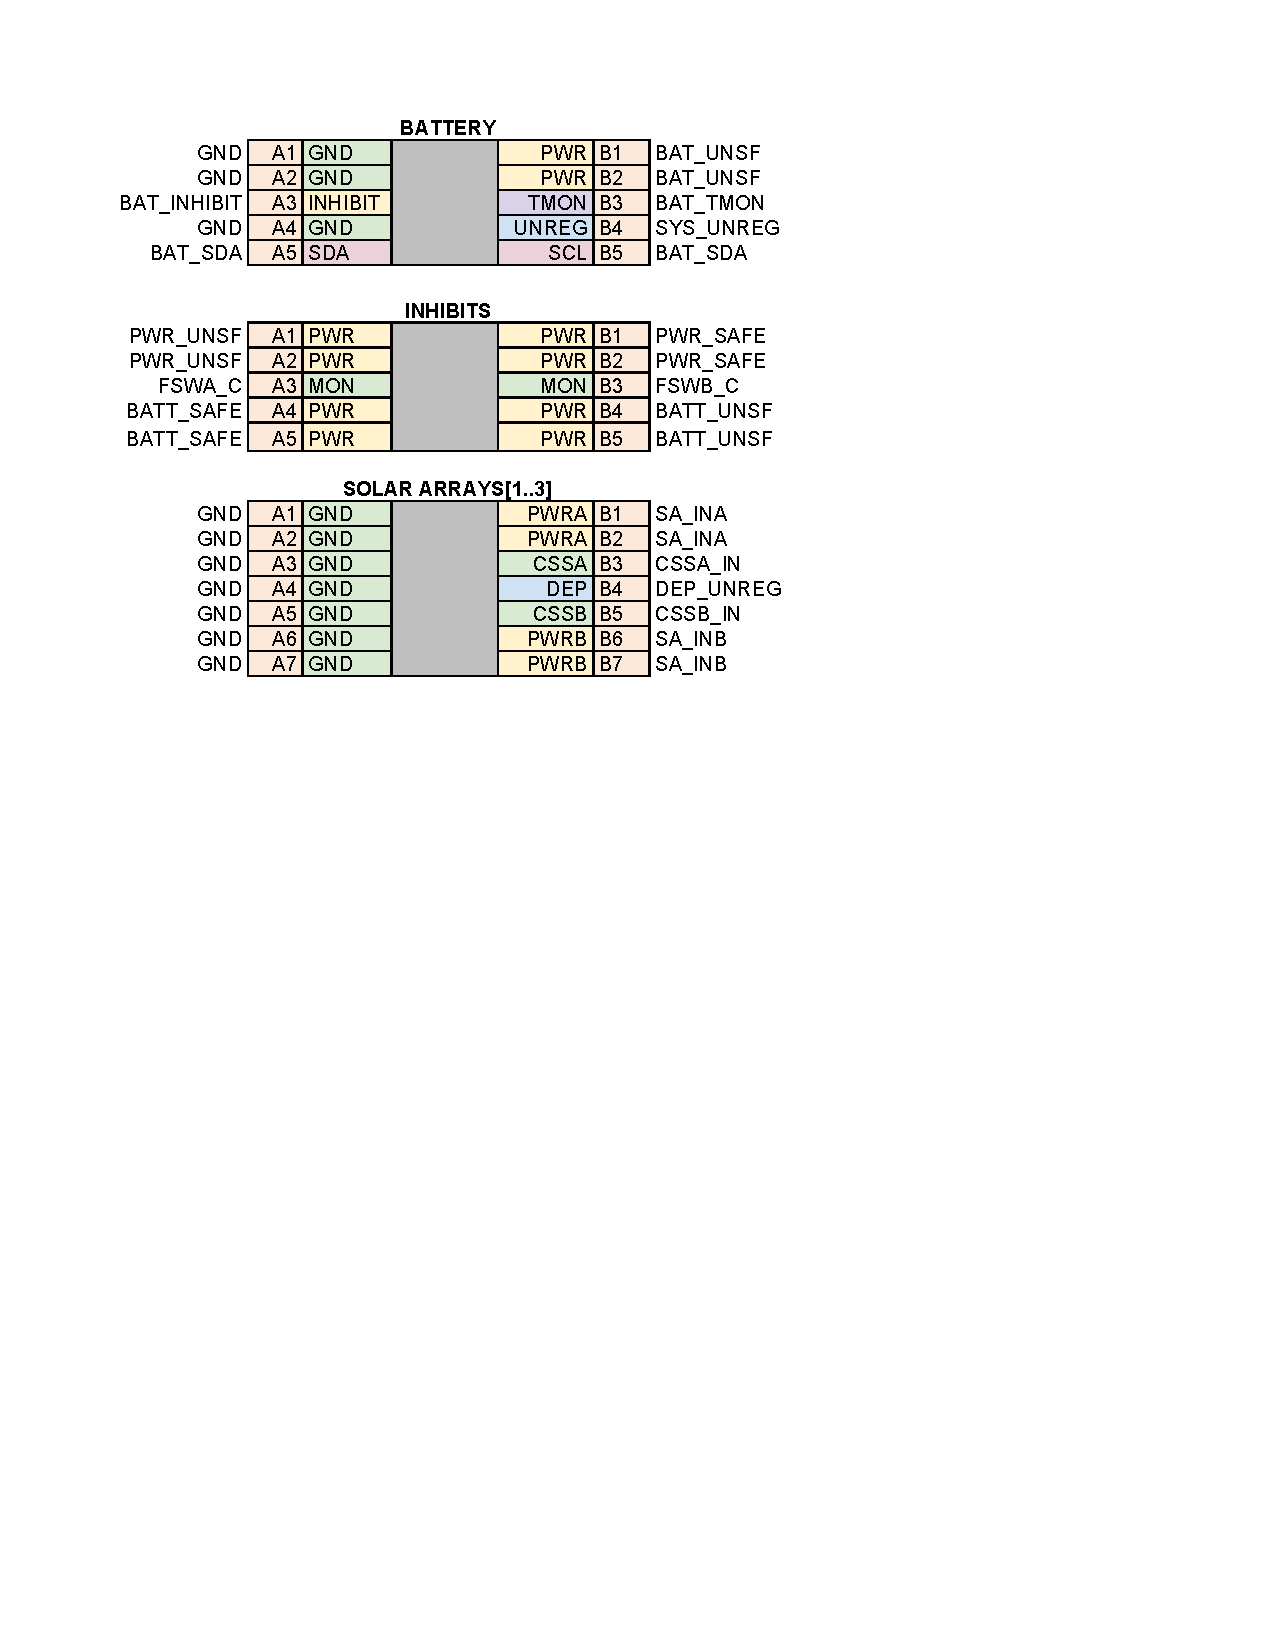
\includegraphics[width=0.5\textwidth]{../figs/phoenix/concept/bat_sa_inh_pins.pdf}
	\caption{New connector pinouts.}
	\label{fig:bat_sa_inh_pins}
\end{figure}

\begin{figure}[htbp]
	\centering
	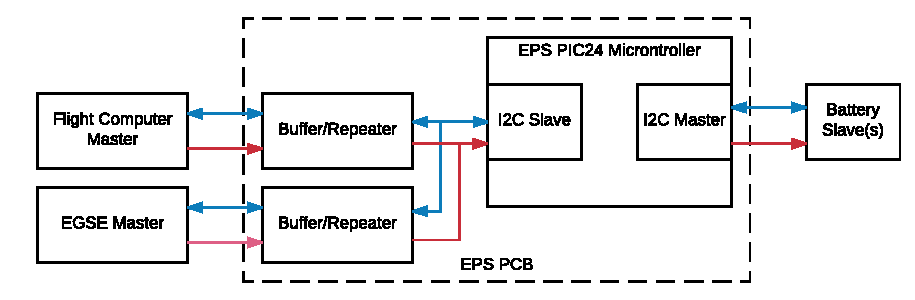
\includegraphics[width=\textwidth]{../figs/phoenix/concept/i2c_tree.pdf}
	\caption{New connector pinouts.}
	\label{fig:i2c_tree}
\end{figure}

\section{Circuit Simulations and Calculations}\label{Sect:eps_calc}



\section{PCB Layout and Mechanical Design}\label{Sect:eps_pcb}



\section{Lessons Learned and Future Work}\label{Sect:eps_results}

In this case, there were several times when the requirements, conceptual design, schematic, and PCB layout were all being updated and altered in parallel. As the IT-SPINS mission and the operation of its subsystems became more fully defined, the critically important EPS design had to be altered to maintain compatibility. In hindsight, these changes made the design method seem somewhat chaotic when 